\documentclass[b5paper,11pt]{article}
\usepackage[colorlinks]{hyperref}
\usepackage{graphicx}
\usepackage{tikz-cd}
\usepackage{notestemplate}
\title{Motivic Homotopy Theory}
\author{Chow.}
\begin{document}
\maketitle
\tableofcontents
	\section{Construction of Unstable Homotopy Category}
	In order to refine the triangulated category of Voevodsky's motives and apply more tools from algebraic topology, we need well-behaved homotopy theory for schemes. Homotopy theory for schemes also allow us to construct motivic cohomology and algebraic K-theory which are looked as generalized cohomology theory defined with Brown representativity theorem.
	\subsection{Simplicial Methods for Algebraic Geometry}
	Let us firstly recall some simplicial homotopy theory.
	$\Delta$ is category consists of objects such as
	\[
	[n]={0 \to 1 \to 2 \to \cdots \to n}
	\]
	for all non-negative integer $n$. And morphisms are functions of sets preserving the order of arrows.
	The category of \emph{simplicial sets} means the category of presheaves on $\Delta$ with values over $\mathbf{Sets}$. It is denoted by $\mathbf{sSets}$.
	
	In category of simplicial sets, we have following canonical objects
	\[
	\Delta[n] := \Delta(-,[n])
	\]
	They are call \emph{standard simplicial sets}.
	\begin{secprop}
		$\Delta([m],[n])$ is generated by following morphisms
		\[
		\begin{aligned}
			d^i \colon [k] &\to [k+1]\\
			d^i(0 \to 1 \to 2 \to \cdots \to k)&=\begin{cases}
			1\to 2 \to \cdots \to k+1& \text{if } i =0\\
			0 \to 1 \to \cdots \to i-1 \to i+1 \to \cdots \to k+1& \text{if } 1\leq i \leq k\\
			0 \to 1 \to \cdots \to k& \text{if } i =k+1\\
			\end{cases}
		\end{aligned} 
		\]
		and
		\[
		\begin{aligned}
		s^i \colon [k] &\to [k-1]\\
		s^i(0 \to 1 \to 2 \to \cdots \to k)&=\begin{cases}
		0\to 0 \to 1 \to \cdots \to k-1& \text{if } i =0\\
		0 \to \cdots \to i \to i  \to \cdots \to k-1& \text{if } 1\leq i \leq k-1\\
		\end{cases}
		\end{aligned} 
		\]
		where $d^i$ is called co-face map and $s^i$ is called co-degeneracy map.
	\end{secprop}
$\Delta$ is small category. As diagram, $\Delta$ looks like
\[
\begin{tikzcd} 
 {[0]} \arrow[r, shift left,"d^0"] \arrow[r, shift right,"d^1"'] & {[1]} \arrow[r,"d^0" description] \arrow[r, shift left=4,"d^1"] \arrow[r, shift right=4,"d^2"'] & \cdots 
\end{tikzcd}
\]
\[
\begin{tikzcd} 
{[0]} \arrow[r,"s^0",leftarrow] & {[1]} \arrow[r,shift left,"s^0",leftarrow] \arrow[r, shift right,"s^1"',leftarrow]  & \cdots 
\end{tikzcd}
\]
By Yoneda lemma, for simplicial set $X \in \mathbf{sSets}$, we have 
\[
X([n])\simeq \mathbf{sSets}(\Delta[n], X)
\]
For convenience, we always denote $X([n])$ by $X_n$ for simplicial set $X$, $d_i = X(d^i)$ and $s_i= X(s^i$). 
\begin{figure}[h]
	\caption{Idea of simplicial sets (from ncatlab)}
\centering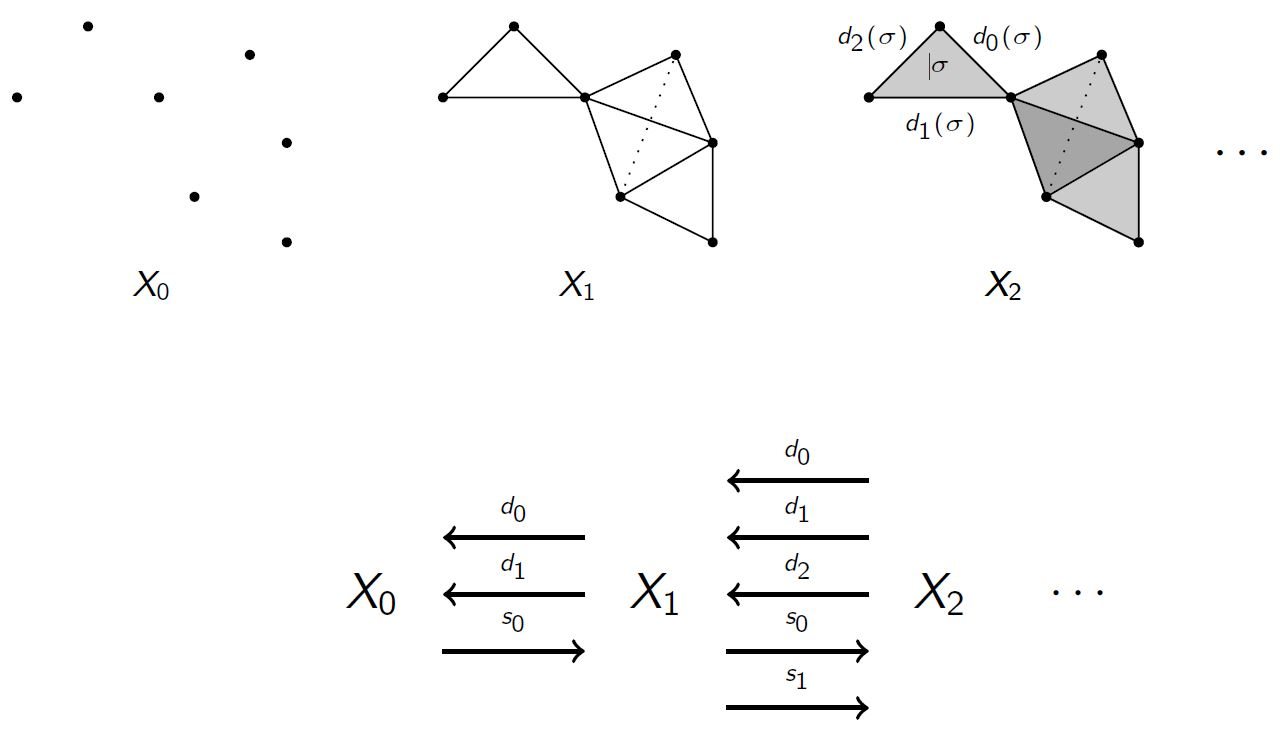
\includegraphics[scale=0.5]{PIC/SimplicialSetsIdea.jpg}
\end{figure}

Let $\Delta^n$ be standard simplex in topological space category. Then we can defined topological space respect to given simplicial set $X$ as follows
\[
|X| := \colim_{(\Delta_n \to X) \in \mathbf{sSets}/X} \Delta^n
\]
Furthermore, $|-|$ is covariant functorial in $\mathbf{sSets}$ since co-representable $\mathbf{sSets}(\Delta_n,-)$ and colimit are functorial. $|-|$ is called \emph{geometric realization functor}.

In classical simplicial homotopy theory, we can endow $\mathbf{sSets}$ with model structure where fibrations are Kan fibrations and weak equivalence are morphisms which induce isomorphisms between fibrant objects on homotopy groups (can be defined as homotopy groups of corresponding geometric realizations).
\subsubsection{Simplicial Objects}
Let $\mathcal{C}$ be arbitrary category. We say $X_*$ is a \emph{simplicial object} on $\mathcal{C}$ if $X_*$ is a presheaf $X_* \colon \Delta^{op} \to \mathcal{C}$ and $\mathbf{s}\mathcal{C}$ denotes the category of simplicial objects on $\mathcal{C}$. Hence simplicial sets are simplicial objects on $\mathbf{Sets}$. 

If $\mathcal{A}$ is  an Abelian category, then we have following correspondence
\begin{secprop}[Dold-Kan Correspondence]
\[
N \colon s\mathcal{A} \to \mathbf{Ch}_{\geq 0} (\mathcal{A})
\]
is equivalence of categories and is also Quillen equivalence (i.e.\ Quillen functor induce equivalence between homotopy categories) with respect to canonical model structure on $s\mathcal{A}$ and projective model on $\mathbf{Ch}_{\geq 0 } (\mathcal{A})$. $N$ is functor of normalized complex and $\mathbf{Ch}_{\geq 0}(\mathcal{A})$ is category of non-negative chain complexes. This equivalence is called \emph{Dold-Kan correspondence}.
\end{secprop}
This proposition means that homological algebra over Abelian category in low bounded case is equivalent to homotopy theory for its simplicial objects. It is convenient to study homotopy theory for simplicial objects because we have geometric realization functor to make constructions more natural. So we can transplant properties from classical homotopy theory into homological algebra.
\subsubsection{Simplicial Homotopy Theory for Presheaves and Sheafification}
Suppose $\mathbf{PSh}^{\mathbf{Sets}}(\mathcal{C})$ be the category of presheaves of sets on $\mathcal{C}$. Then the associated category of simplicial objects $s\mathbf{PSh^{Sets}}(\mathcal{C})$ is isomorphic to $\mathbf{PSh^{sSets}}(\mathcal{C})$ --- the category of presheaves of simplicial sets on $\mathcal{C}$. Let $X_* \in s\mathbf{PSh^{Sets}}(\mathcal{C})$
\[
F_* \mapsto F
\]
where \[
F(X)_n := F_n(X) \ \forall X \in \mathcal{C}
\]
In this case, $s\mathbf{PSh^{Sets}}(\mathcal{C})$ or $\mathbf{PSh^{sSets}}(\mathcal{C})$ is called category of simplicial presheaves of sets on $\mathcal{C}$.

$\mathbf{PSh^{sSets}}(\mathcal{C})$ can be endowed with model structure objectwise by model structure of $\mathbf{sSets}$.
\begin{itemize}
	\item $\alpha \colon F \Rightarrow G$ is weak-equivalence if and only if for all $X \in \mathcal{C}$, $\alpha_X: F(X) \to G(X)$ is weak-equivalence in $\mathbf{sSets}$.
	\item $\beta\colon F \Rightarrow G$ is fibration if and only if for all $X \in \mathcal{C}$, $\beta_X$ is Kan fibration.
\end{itemize}
Then the model structure of $\mathbf{PSh^{sSets}}(\mathcal{C})$ is fibrantly generated. This model structure on $\mathbf{PSh^{sSets}}(\mathcal{C})$ is called \emph{global model structure}.

If $\mathcal{C}$ is a site with Grothendieck topology, we can define $\mathbf{Sh^{sSets}_\tau} (\mathcal{C})$ be the category of $\tau$-sheaves of sets on $\mathcal{C}$ and $\mathbf{PSh_\tau^{sSets}}(\mathcal{C})$ the category of simplicial presheaves with model structure called \emph{$\tau$-local model structure} as follows. 
\begin{secdefn}[$\tau$-local weak equivalence]
	A \emph{$\tau$-local weak equivalence} is a morphism between presheaves $f \colon F \Rightarrow G$ such that
	\begin{itemize}
		\item The morphism induces isomorphism $\tilde{\pi}_0(f): \tilde{\pi}_0X \to \tilde{\pi}_0Y$ in $\mathbf{Sh^{Sets}}(\mathcal{C})$;
		\item For all $U \in \mathcal{C}$, $\tilde{\pi}_n(f): \tilde{\pi}_n(X,x) \to \tilde{\pi}_n(Y,f(x))$ is isomorphism on $\mathcal{C}/U$ for any choice of base point $x \in X(U)$.
	\end{itemize}
\end{secdefn}
The $\tau$-local cofibrations are same as ordinary cofibrations of $\mathbf{PSh^{sSets}}(\mathcal{C})$ and $\tau$-fibrations are morphisms in $\mathbf{PSh^{sSets}}(\mathcal{C})$ satisfy RLP for $\tau$-acyclic cofibration (i.e.\ be both $\tau$-cofibration and $\tau$-weak equivalence).

In particular, if $\mathcal{C}=(Sm/S)_\tau$ is site of smooth $S$-schemes with Grothendieck topology $\tau$, we denote $\mathbf{Spc}^{pre}(S)$ (resp.\ $\mathbf{Spc}_\tau^{pre}(S)$, resp.\ $\mathbf{Spc}_\tau(S)$) the category of simplicial presheaves (res.\ simplical presheaves with $\tau$-local model structue, resp.\ simplicial $\tau$-sheaves) on $\mathcal{C}=(Sm/S)_\tau$. $\mathbf{Spc_\tau}(S)$ is full subcategory of $\mathbf{Spc}^{pre}_\tau(S)$ and left adjoint functor $s$ of inclusion exists. This fucntor is called is called \emph{sheafification functor} under topology $\tau$. Hence $\mathbf{Spc_\tau}(S)$ is model category. Furthermore, we have 
\begin{secprop}
	The pair $(s ,i)$ of adjunction is a pair of Quillen equivalence.
\end{secprop}
Hence we have $\mathbf{Ho}(\mathbf{Spc}_\tau^{pre}(S)) \simeq \mathbf{Ho}(\mathbf{Spc}_\tau(S))$, denoted by $\mathcal{H}_\tau(S)$.
\subsubsection{Hypercovers and Bousfield localization}
More generally, we can realize $\tau$-local model structure on $\mathbf{PSh^{sSets}_\tau}(\mathcal{C})$ as Bousfield localization with respect to $\tau$-hypercovers.
\begin{secdefn}[Bousfield localization]
	
\end{secdefn} 
\end{document}